
\chapter{Background}
\label{chap:background}

This chapter explains the basic concepts used throughout the thesis.

In \autoref{sec:lms}, we first cover \emph{neural \acp{lm}}. We start with a brief theory of neural networks and text representation for neural networks. This theoretical grounding will help us to define the task of language modeling and its connection to neural networks. We then look at specific neural architectures, particularly the transformer architecture, and show how pretraining models based on this architecture can produce models with strong \ac{nlp} capabilities.

In \autoref{sec:d2t}, we turn our attention to \ac{d2t} generation, the central task explored in this thesis. To motivate the task, we start with an overview of real-world \ac{d2t} applications. We also explain the subtasks into which \ac{d2t} generation can be decomposed. We show how various approaches tackle these subtasks, starting from early rule-based approaches to recent neural-based systems. Finally, we describe \ac{d2t} datasets and evaluation metrics, focusing on the ones relevant to this thesis.

We assume that the typical reader of this thesis comes from a related \ac{nlp} area and is familiar with the relevant concepts. That being said, the thesis can also be used by a beginner in the field, as the work is self-contained and provides pointers to relevant work for more details. The chapter serves as the main point of reference; we will only briefly revisit the most relevant concepts in the respective chapters.




\section{Neural Language Models}
\label{sec:lms}
In this section, we work our way towards neural \acp{lm}. We start with the mathematical foundations of \acp{nn} on which the neural \acp{lm} are built (\autoref{sec:nns}), the ways we can represent text in neural networks (\autoref{sec:text-repr}), and the basic ideas of language modeling (\autoref{sec:lm-basics}). Equipped with the necessary theoretical background, we then introduce the transformer architecture (\autoref{sec:transformer}) and how it serves as a basis for pretrained (\autoref{sec:plms}) and large (\autoref{sec:llms}) language models.

\subsection{Neural Networks}
\label{sec:nns}
Neural networks are a tool for learning patterns from data.\footnote{Until we get to \ac{d2t} generation in \autoref{sec:d2t}, we use the word ``\textit{data}'' only in its abstract sense, as in ``any inputs we can apply our algorithms to''. We use the term ``structured data'' whenever it is necessary to make the distinction.} Such a tool will help us with learning language patterns from large-scale textual data, and in turn with generating text.

To begin, let's say our goal is to predict real-number output $y \in \mathbb{R}$ for the given vector of real numbers $\mathbf{x} = (x_1, \ldots, x_d) \in \mathbb{R}^d$.
% \footnote{We will follow the convention that vectors are denoted with boldface letters ($\mathbf{x}$), and real numbers with plain letters ($x$).} 
We assume that the $\mathbf{x} \rightarrow y$ mapping is not arbitrary---that would leave us with memorizing all the $(\mathbf{x},y)$ pairs---but follows some regularities and underlying patterns that can be learned. This assumption is naturally satisfied if we consider $(\mathbf{x},y)$ to be representations of real-world data, e.g., documents and their labels.

We use mathematical models designed to capture the patterns in their parameters to learn the mapping. The models estimate the parameters from a set of $(\mathbf{x},y)$ examples called the \textit{training data} and use the parameters to predict the outputs on a separate set of examples (generally assumed to come from the same data-generating distribution) called the \textit{test data}.

\paragraph{Perceptron Algorithm} One of the early mathematical models designed for learning patterns from data is the \emph{perceptron algorithm} (\citealp{rosenblatt1958perceptron}, \citealp[p.~192]{bishop2006pattern}). For the perceptron algorithm, we need to restrict the output to a binary class label: $y \in \{-1, 1\}$. The algorithm learns the parameters $\textbf{w} = (w_1, \ldots, w_d) \in \mathbb{R}^d$ and the bias $b \in \mathbb{R}$ describing a linear decision boundary separating the data points according to their class label. The algorithm proceeds as follows:


\begin{enumerate}
    \item The parameters $\textbf{w}$ and $b$ are initialized to small random values (or zeros).
    \item For each training example $(\mathbf{x}_i, y_i)$, the algorithm updates the weights and bias to adjust their current estimate $\hat{y}_i$ towards the ground truth target $y_i$:
          \begin{align} \label{eq:perceptron1}
              \hat{y}_i  & = \text{sign}(\textbf{w} \cdot \mathbf{x} + b) \\
              \textbf{w} & = \textbf{w} + (y - \hat{y}) \textbf{x}        \\
              b          & = b + y - \hat{y}
          \end{align}
    \item The step (2) is repeated until convergence.
\end{enumerate}

The perceptron algorithm is guaranteed to converge if a hyperplane exists that separates the data belonging to one class from another; otherwise, it does not converge \cite{novikoff1962convergence}.

\paragraph{Multi-layer Perceptron} To overcome the fact that the perceptron is limited to linear decision boundaries, we can use a \emph{\acl{mlp}} (\acs{mlp}\glsunset{mlp}; \citealp[p.~164]{goodfellow2016deep}). This mathematical model---also known as a \emph{feed-forward neural network}---can approximate any bounded continuous function \cite{hornik1989multilayer}.

As the name suggests, \ac{mlp} processes the input with multiple perceptron-like units called \textit{neurons}. Analogically to the perceptron (\autoref{eq:perceptron1}), each neuron computes its output $o$ using the rule:
\begin{align}
    o & = f(\mathbf{x}^\top \mathbf{w}  + b),
\end{align}
where $f: \mathbb{R} \rightarrow \mathbb{R}$ is the \emph{activation function}, $\mathbf{x}\in \mathbb{R}^n$ is the input vector, and $\mathbf{w} \in \mathbb{R}^n$ and $b \in \mathbb{R}$ are learnable parameters. Instead of signum, \ac{mlp} uses differentiable non-linear functions, nowadays most commonly the \acl{relu} (\acs{relu}\glsunset{relu}; \citealp{nair2010rectified}), where $f(x) = \text{max}(0, x)$, or its variants \cite{hendrycks2016gaussian,dubey2022activation}.

For efficiency, the neurons are organized in layers, which enables formulating \ac{mlp} computations in terms of matrix multiplication. The $i$-th layer of \ac{mlp} is parametrized with a matrix $\mathbf{W}_i \in \mathbb{R}^{d\times n}$ and a vector of biases $\mathbf{b}_i \in \mathbb{R}^{n}$, processing the intermediate output called the \textit{hidden state} $\mathbf{h}_{i-1} \in \mathbb{R}^{d}$ (where we set $\textbf{h}_0 = \textbf{x}$):
\begin{align}
    \mathbf{h}_i & = f(\mathbf{h}_{i-1} \mathbf{W}_i + \mathbf{b}_i).
\end{align}

To estimate the parameters of the network, we need to \emph{train} the network using the training data. For each training example $(\mathbf{x}, y)$, we first do a \emph{feed-forward pass}: we feed $\mathbf{x}$ into the network and use the current parameters of the network to get the prediction $\hat{y}$. We then update the parameters to minimize the gap between the predicted output $\hat{y}$ and the ground truth output $y$. This gap is described by a \textit{loss function} $\mathcal{L}(y, \hat{y}) \rightarrow \mathbb{R}$.
Since all the computations in \ac{mlp} are differentiable, we can compute exactly how much each parameter contributes to the loss function using the chain rule for derivatives. The derivative for each parameter---called a \emph{gradient} when grouped in a vector---directly influences the size of the update. The process of computing and applying the updates is called a \emph{backward pass} (or backpropagation; \citealp{kelley1960gradient,rumelhart1986learning}) and operates in the reverse order of layers. The magnitude of the updates is controlled by the \emph{learning rate} $\alpha \in \mathbb{R}$.

One of the basic optimizers (i.e., the algorithms for updating the parameters) is the {\acl{sgd} (\acs{sgd}\glsunset{sgd}; \citealp[p.~275]{goodfellow2016deep}). SGD estimates the gradient in each step using a limited number of examples called a \emph{batch} and directly updates the parameters in the direction of the gradient. More advanced optimizers, such as Adam \cite{kingma2014adam}, also adapt the learning rate for each parameter based on the history of the gradients, helping to make the convergence more robust.

\paragraph{Recurrent Neural Networks} Unlike with \acp{mlp}, where we the size of the input is fixed, \acp{rnn} allow us to process a sequence of inputs $\mathbf{X} = (\mathbf{x}_1, \ldots, \mathbf{x}_n)$ of arbitrary length. An \ac{rnn} computes a sequence of hidden states $\mathbf{H} = (\mathbf{h}^{(0)}, \ldots, \mathbf{h}^{(n)})$, i.e., one state for each input in the sequence. $\mathbf{H}$---or sometimes more specifically, the last hidden state $\mathbf{h}^{(n)}$---is the encoded representation of the input sequence, which can be in turn used in downstream tasks (e.g., for tagging or classifying the sequence).

The \ac{rnn} computes the hidden states $\mathbf{H}$ by repeatedly applying a function $f$ parametrized by the parameters of the network $\boldsymbol{\theta}$, the current input $\mathbf{x}_i$, and the previous hidden state $\mathbf{h}^{(i-1)}$ \cite[p.~367]{goodfellow2016deep}:
\begin{align}
    \mathbf{h}^{(i)} = f(\boldsymbol{\theta}, \mathbf{h}^{(i-1)}, \mathbf{x}_i),
\end{align}
where the first hidden state $\mathbf{h}^{(0)} \in \mathbb{R}^k$ is initialized randomly.  The function $f$ is generally implemented as a series of matrix multiplications and non-linear functions. The exact implementation of $f$ can get more complex with advanced \ac{rnn} architectures such as LSTM \cite{hochreiter1997long} or GRU \cite{cho2014learning}.

\acp{rnn} had various successes across \ac{nlp} on sequence processing tasks \cite{karpathy2015unreasonable,salehinejad2017recent}. At the same time, \acp{rnn} turned out to have various shortcomings, such as the vanishing gradient problem, the fixed size of the hidden state, and limited possibilities of parallelization; all of which made it hard to model long-term dependencies and train the network efficiently \cite{hochreiter1998vanishing,pascanu2013difficulty}. We return to \acp{rnn} mainly in \autoref{sec:transformer}, showing how it became a predecessor to the transformer architecture.


\subsection{Text Representation}
\label{sec:text-repr}
In this section, we look into how we can represent text in neural networks.

\paragraph{One-Hot Encoding}
% Until now, we have assumed that the input to a network is a vector of real numbers. However, a
A text is a sequence of discrete units such as characters or words. To convert these units---called \textit{tokens}---to a numerical representation, we first enumerate a set of all possible tokens (a \textit{vocabulary} $V$) and assign each token an integer index $i \in \{0, \ldots, |V|-1\}$.

The naive way to represent each token would be using its integer value. However, this would misleadingly suggest linear dependence between tokens. A better way is to use the index $i$ for constructing a \textit{one-hot} vector $\mathbf{x} \in \{0,1\}^{|V|} $ for each token:
\begin{align}
    x_j = \begin{cases}
        1 & \text{if } i = j, \\
        0 & \text{otherwise}.
    \end{cases}
\end{align}
While this representation is more sound, it is quite sparse and does not capture the semantics of individual tokens, which puts high requirements on the representational capacity of the network.

\paragraph{Word Embeddings} A more useful representation of tokens is the one in which the tokens with similar meanings are also close in the vector space. To get this representation, we can build on the distributional theory of meaning, according to which the meaning of a token is defined by a context in which it occurs \cite{harris1954distributional,firth1957synopsis}.
% A straightforward implication of the theory is that the tokens with similar meanings tend to occur in similar contexts. 

In the context of neural networks, this idea is used in the Word2Vec algorithm \cite{mikolov2013distributed}. The algorithm trains an \ac{mlp} for a specific objective and uses its weigths as token representations. The \ac{mlp} training objective (illustrated in \autoref{fig:word2vec}) either consists of predicting the tokens in the neighborhood of each token (the \emph{skip-gram} objective) or vice versa, the token itself based on the tokens in its neighborhood (the \emph{continuous bag-of-words} objective). The output of the algorithm is an \textit{embedding matrix} $\mathbf{W}_e \in \mathbb{R}^{|V|\times d}$, which assigns each token a $d$-dimensional \textit{embedding vector} $\mathbf{x} \in \mathbb{R}^{d}$.

\begin{figure*}[ht]
    \centering

    \begin{subfigure}{\textwidth}
        \centering
        \begin{subfigure}{0.45\textwidth}
            \centering
            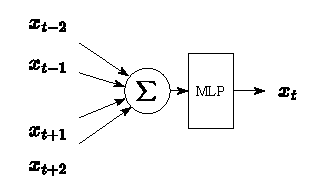
\includegraphics[width=\textwidth]{img/skipgram.pdf}
            \caption{Skip-gram}
            \label{fig:skipgram}
        \end{subfigure}
        \hspace{-20px}
        \begin{subfigure}{0.45\textwidth}
            \centering
            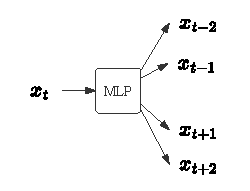
\includegraphics[width=0.75\textwidth]{img/cbow.pdf}
            \caption{Continuous Bag-of-Words}
            \label{fig:cbow}
        \end{subfigure}
    \end{subfigure}
    \caption{The objectives employed by the Word2Vec algorithm \cite{mikolov2013distributed}. The algorithm here uses a context window of size $k=5$. In the (a) \emph{skip-gram} algorithm, we sum the embeddings of $k-1$ surrounding tokens and predict the original token. In the (b) \emph{continuous bag-of-words} algorithm, we use the original token for predicting the $k-1$ surrounding tokens.}
    \label{fig:word2vec}
\end{figure*}

The notion of using an embedding matrix for representing tokens is used also in neural \acp{lm} (\autoref{sec:lm-basics}). However, in majority of neural \acp{lm}, the embedding matrix is not trained separately with a specific algorithm, but jointly with the rest of the network.

\paragraph{Tokenization} Until now, we have implicitly assumed that we have a way of tokenizing the text, i.e. splitting it into discrete units. The most straightforward way is to tokenize the text into words or characters. However, these approaches have major shortcomings. Word-level tokenization considers morphologically similar words as independent units, forcing the model to learn their representation separately. It also becomes more difficult for languages such as Chinese, which do not separate words with spaces. In contrast, character-level tokenization is computationally inefficient and gives us less meaningful units.

\emph{Subword tokenization}  is the middle ground between the word-level and character-level tokenization. It splits the text into smaller pieces called \emph{subwords}, which are continous character spans of various length. With subword tokenization, frequently used words typically get their own subword while less frequent words are split into multiple subwords.

The subword tokenization algorithm that is commonly used in neural \acp{lm} is \emph{\acl{bpe}} (\acs{bpe}\glsunset{bpe}; \citealp{sennrich2016neural}). The \ac{bpe} algorithm starts with the vocabulary of individual bytes, iteratively merging the most frequent tokens and adding them to the vocabulary $V$ until we reach the target vocabulary size. An example subword tokenization of the expression ``Subword tokenization'' could be the subwords \texttt{ ['Sub', 'word', '▁token', 'ization']}, where ``\texttt{▁}'' is a special character denoting a preceding space.


\subsection{Language Modeling}
\label{sec:lm-basics}
After establishing the theory of neural networks and showing how to represent text in neural networks, we are ready to explain the notion of \emph{language modeling}, a central concept for building neural \acp{lm}.

\paragraph{Language Model} A \emph{language model} is a mathematical model that estimates a probability of a sequence of tokens $X = (x_1, \ldots, x_n)$. To estimate the probability, we can factorize the sequence probability using the chain rule:
\begin{align}
    P(X) = \prod_{i=1}^n P(x_i|x_1, \hdots, x_{i-1}).
\end{align}
This formulation gives us a way to compute the probability of the whole sequence as the product of probabilities of individual sequence prefixes.

\paragraph{\emph{n}-gram Language Model} An \emph{n}-gram \ac{lm} (parametrized by a positive integer $n$) further simplifies the product using the assumption that the probability of a token depends only on $N-1$ previous tokens \cite[p.32]{jurafsky2024}:
\begin{align}
    P(X) = \prod_{i=1}^T P(x_i|x_{i-N+1}, \hdots,x_{i-1}).
\end{align}
The probabilities for individual \emph{n}-grams are estimated by counting their occurrences over a text corpus, storing the counts in a look-up table. The main limitation of $n$-gram \acp{lm} (besides the size of the look-up tables) is the limit on the length of the context for each token, due to which \emph{n}-gram \acp{lm} fail to capture long-term dependencies.




\paragraph{Neural Language Model} A neural \ac{lm} is a \acl{lm} that estimates the text probability $P_\theta(X)$ using a neural network with parameters $\theta$. In contrast with \emph{n}-gram \acp{lm}, neural \acp{lm} can capture long-term dependencies and efficiently store the probability distribution in their parameters.

The parameters of the neural \ac{lm} are also estimated using a text corpus. For each word $x_i$ in the corpus, we aim to maximize the conditional probability that the model assigns to the word $P_\theta(x_i|x_{<i})$. If we express the gap between the model distribution $P_\theta$ and the empirical distribution of sequences in the corpus $P$ using cross entropy, this formulation is equal to minimizing the negative log-likelihood of the next word \cite[p.158]{jurafsky2024}:
\begin{align}
    \mathcal{L}_{CE} = - \log P_\theta(x_i|x_{<i}).
\end{align}

This type of training is also called \emph{self-supervised}: each token in the corpus serves as the ground-truth label that the model aims to predict. We discuss the training objectives for specific model architectures in \autoref{sec:plms}.


\subsection{Transformer Architecture}
\label{sec:transformer}
In this section, we pave the way towards the \emph{transformer} \cite{vaswani2017attention}: the core neural architecture used in \ac{nlp} nowadays. We describe its individual components and how the transformer is used for text processing.

\paragraph{Encoder-Decoder Framework}
We have described the \ac{rnn} (\autoref{sec:nns}) as a neural network that can \emph{encode} an input sequence into hidden states. The encoder-decoder framework \cite{sutskever2014sequence,cho2014learning} allows us to also \emph{generate an output sequence}. The idea is to use another network called the \emph{decoder} for generating the sequence, using the last hidden state of the encoder as its initial state. Here, we illustrate how the framework is applied using two \acp{rnn}:\footnote{Later adapting the general idea also for the transformer architecture.}

\begin{enumerate}
    \item The \ac{rnn} called the \emph{encoder} encodes the sentence of input embeddings $\mathbf{X}= (\mathbf{x}_1, \ldots, \mathbf{x}_n)$ into a sequence of hidden states $\mathbf{H}_e = \{\mathbf{h}_e^{(0)}, \ldots, \mathbf{h}_e^{(n)}\}$ (where $\mathbf{h}_e^{(0)}$ is a null vector) by repeatedly applying a transformation $\mathcal{E}$ in each timestep $i\in(1,n)$:
          \begin{align}
              \mathbf{h}_e^{(i)} = \mathcal{E}(\mathbf{h}_e^{(i-1)}, \mathbf{x}_i).
          \end{align}
    \item The \ac{rnn} called the \emph{decoder} uses $\mathbf{h}_e^{(n)}$ as its initial state $\mathbf{h}_d^{(0)}$ and produces the sequence of output tokens  $Y = (y_1, \ldots, y_m)$ by repeatedly applying a transformation $\mathcal{D}$ in each timestep $j\in(1,m)$:
          \begin{align}
              \mathbf{h}_d^{(j)}, y_j = \mathcal{D}(\mathbf{h}_d^{(j-1)}, y_{j-1}).
          \end{align}
\end{enumerate}

Note that the decoder produces the output sequence iteratively, yielding a token $y_j$ in each timestep. This process is called \emph{autoregressive decoding} and is described in more detail in \autoref{sec:plms}.

\paragraph{Attention Mechanism} We have mentioned that the hidden state of an \ac{rnn} has a fixed size, which limits the amount of information the network can capture about a sequence. The \emph{attention mechanism} \cite{bahdanau2015neural} enables the decoder to extract the information dynamically from the encoded sequence. In each step $j$, the decoder computes a context vector $c_j$ as the weighted sum of the hidden states of the encoder $\mathbf{H}_e$ using the attention matrix $\mathbf{W}_a$:
\begin{align}
    \alpha_{ji}  & = \operatorname{softmax}(\mathbf{h}_d^{(j)}\mathbf{W}_a \mathbf{h}_e^{(i)}), \\
    \mathbf{c}_j & = \sum_i \alpha_{ji} \mathbf{h}_e^{(i)}.
\end{align}
The context vector is used as an additional input for the decoder:
\begin{align}
    \mathbf{h}_d^{(j)}, y_j = \mathcal{D}(\mathbf{h}_d^{(j-1)}, y_{j-1}, \mathbf{c}_j).
\end{align}


\paragraph{Self-attention Mechanism} Self-attention \cite{cheng2016long,vaswani2017attention} is a variant of the attention mechanism in which the source and the target sequence are identical. Given the input $\mathbf{X} \in \mathbb{R}^{n,d}$, the \emph{self-attention} produces the output $\mathbf{H} \in \mathbb{R}^{n,d}$ of the same size. For each token, the resulting vector $\mathbf{h}_i \in \mathbf{H}$ is a weighted combination of the value vectors corresponding to all the tokens in a sequence (including the token itself):
\begin{align}
    \mathbf{h}_j = \sum_{i\in 1..n} \alpha_{ji} \mathbf{v}_i,
\end{align}
where the \emph{value vector} of each token is computed using a trainable \emph{value matrix} $\mathbf{W_v} \in \mathbb{R}^{n,d}$:
\begin{align}
    \mathbf{v}_i = \mathbf{x}_i \mathbf{W_v}.
\end{align}
To get the attention weights $\alpha_{ij}$, we first compute \textit{query} and \textit{key} vectors for each token using trainable matrices $\mathbf{W_q}$ and $\mathbf{W_k} \in \mathbb{R}^{n,d}$. Each weight is a normalized dot product of the corresponding vectors:
\begin{align}
    \mathbf{q}_i & = \mathbf{x}_i \mathbf{W_q}                                                      \\
    \mathbf{k}_i & = \mathbf{x}_i \mathbf{W_k}                                                      \\
    \alpha_{ij}  & = \operatorname{softmax}\biggl(\frac{\mathbf{q}_i\mathbf{k}_j}{\sqrt{d}}\biggr).
\end{align}
The operations can be efficiently parallelized using matrix multiplication:
\begin{align}
    \mathbf{Q}                                             = \mathbf{X}\mathbf{W_q},\quad\mathbf{K} & = \mathbf{X}\mathbf{W_k},\quad\mathbf{V} = \mathbf{X}\mathbf{W_v}                           \\
    \operatorname{Attn}(\mathbf{Q}, \mathbf{K}, \mathbf{V})                                         & = \operatorname{softmax}\biggl(\frac{\mathbf{Q}\mathbf{K}^\top}{\sqrt{d}}\biggr)\mathbf{V}.
\end{align}


\begin{figure*}[ht]
    \centering
    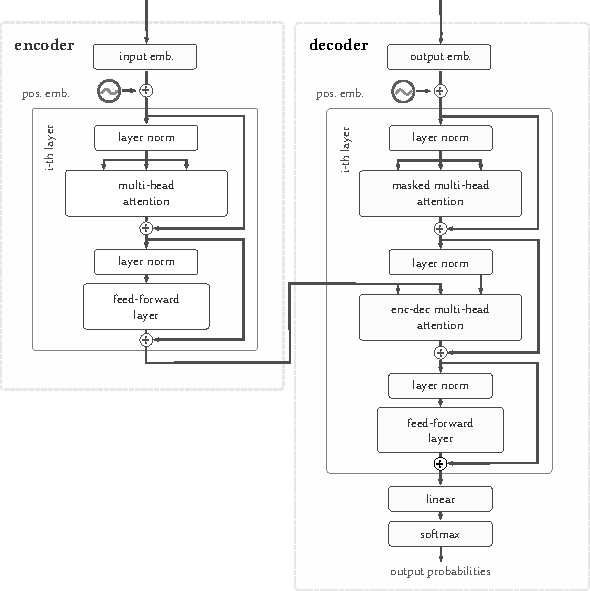
\includegraphics[width=0.9\textwidth]{img/transformer.pdf}
    \caption{An encoder-decoder variant of the Transformer architecture. The encoder has $N_{e}$ layers, each consisting of a self-attention and MLP sublayer. The decoder has $N_{d}$ layers with masked self-attention and encoder-decoder attention, again followed by an MLP sublayer. The input to each sublayer is normalized using layer norm. After the last decoder layer, the output probabilities are computed using a linear projection and softmax. The figure is adapted from \href{https://github.com/bbycroft/llm-viz/blob/main/src/llm/intro-image.svg}{https://github.com/bbycroft/llm-viz}.}
    \label{fig:transformer}
\end{figure*}


\paragraph{Transformer Architecture} The \emph{transformer}\footnote{Although \citet{vaswani2017attention} use ``Transformer'' with a capital ``T'', the orthography is gradually shifting towards the variant with a lower-case ``t''. See, e.g., \citet[p.~215]{jurafsky2024}.} \cite{vaswani2017attention} is a neural network architecture that can process sequences efficiently in parallel. To achieve that, the transformer replaces the \ac{rnn} hidden state (previously used for sharing information among tokens in a single sequence) with the self-attention mechanism applied over a series of layers.

Specifically, each layer is composed of two sublayers: (a) the \emph{self-attention layer} and (b) the \emph{\ac{mlp} layer}. The output of the $i$-th sublayer is added to its original input $\mathbf{H}^{(i)}$ in a \emph{residual connection}:
\begin{align}
    \mathbf{H}^{(i+1)} = \mathbf{H}^{(i)} + \operatorname{sublayer}(\mathbf{H}^{(i)}).
\end{align}
The sublayers serve a different purpose: while the \ac{mlp} layer computes element-wise operations over each token, the self-attention layer enables sharing information among tokens. The sublayer input (or output, depending on the architecture variant) is normalized using \emph{layer normalization} \cite{ba2016layer}.

To get the input representation $\mathbf{H}^{(0)}$, we sum the token embeddings $\mathbf{X} \in \mathbb{R}^{n,d}$ with \emph{positional embeddings}. Positional embeddings encode the absolute or relative position information of individual tokens, which needs to be represented explicitly in parallel processing.\footnote{There are multiple variants of positional embeddings with various trade-offs; see \citet{dufter2022position} for an overview.}


% We train the model on \emph{batches} of data, using an optimization algorithm such as \acl{sgd} (\acs{sgd}\glsunset{sgd}; \citealp[p.~275]{goodfellow2016deep}) or Adam \cite{kingma2014adam}. The batch size $b$ and the learning rate $\alpha$ are the training hyperparameters.
As shown in \autoref{fig:transformer}, the original Transformer architecture is based on the encoder-decoder framework. The decoder layers implement two additional features:
\begin{itemize}
    \item Each layer contains an additional sublayer called the \emph{encoder-decoder attention}. In contrast to the self-attention mechanism, the \emph{keys} and \emph{values} come from the last layer of the encoder, enabling the decoder to attend to the encoded sequence.
    \item The self-attention is \emph{masked} so that each token can collect information only from the preceding tokens, which is necessary to enable training the model for left-to-right autoregressive decoding.
\end{itemize}
After the last decoder layer, the hidden states are projected into a matrix of size $\mathbb{R}^{|V|\times n}$ and normalized using softmax, producing a probability distribution over the vocabulary for each input token.

\subsection{Pretrained Language Models}
\label{sec:plms}
To achieve good performance on downstream tasks, we typically need to spend extensive time for training the transformer on large-scale training data. A more efficient workflow is as follows: the models are first \emph{pretrained} using a generic objective on large-scale data---such as The Pile \cite{gao2020pile}, or C4 \cite{raffelExploringLimitsTransfer2019}---and then \emph{finetuned} for downstream tasks on a smaller, task-specific dataset. Although pretraining a model still requires significant computational resources, \acp{plm} can be then distributed for further finetuning, which is in itself much more efficient.


\begin{table}[t]
    \footnotesize
    \centering
    \begin{tabular}{lp{4.5cm}ll}
        \toprule
        \textbf{Type}            & \textbf{Pretraining Objective}            & \textbf{Model}                                       & \textbf{\# Parameters} \\
        \midrule
        \multirow{2}{*}{Encoder} & \multirow{2}{*}{Masked Language Modeling} & BERT \cite{devlinBERTPretrainingDeep2019}            & 110M-340M              \\
                                 &                                           & RoBERTa \cite{liuRoBERTaRobustlyOptimized2019}       & 125M-355M              \\
                                 &                                           & \textsc{LaserTagger} \cite{malmi2019lasertagger}     & 110M                   \\
        \midrule
        \multirow{2}{*}{Enc-Dec} & \multirow{2}{*}{Text Denoising}           & BART \cite{lewisBARTDenoisingSequencetoSequence2019} & 139M-406M              \\
                                 &                                           & mBART \cite{liuMultilingualDenoisingPretraining2020} & 680M                   \\
                                 &                                           & T5 \cite{raffelExploringLimitsTransfer2019}          & 220M-11B               \\
        \midrule
        Decoder                  & Causal Language Modeling                  & GPT-2 \cite{radfordLanguageModelsAre2019}            & 117M-1.5B              \\
                                 &                                           & Llama2 \cite{touvronLlamaOpenFoundation2023}         & 7B-70B                 \\
                                 &                                           & Mistral \cite{jiangMistral7B2023}                    & 7B-70B                 \\
                                 &                                           & Zephyr \cite{tunstallZephyrDirectDistillation2023}   & 7B-70B                 \\
        \bottomrule
    \end{tabular}
    \caption{Types of transformer architectures and specific models used in this work. The number of parameters may vary based on the model variant.}
    \label{tab:pretrained_models}
\end{table}


\paragraph{Model types} Depending on the downstream task, different variants of the transformer architecture are used (see \autoref{tab:pretrained_models} for an overview):

\begin{itemize}
    \item \textbf{Encoder models} use only the \emph{encoder} part of the transformer architecture. These models are not generative; instead, the models produce a contextualized representation of the input sequence $\mathbf{X}$. The representation can be used for downstream tasks such as sequence classification, sequence tagging, or computing sequence similarity.
    \item \textbf{Encoder-decoder models} use the original \emph{encoder-decoder} architecture, and are explicitly trained to transform an input sequence $\mathbf{X}$ into a target sequence $\mathbf{Y}$. Encoder-decoder models are mostly used for sequence-to-sequence tasks, such as \ac{mt}, question answering, or summarization.
    \item \textbf{Decoder models} use only the \emph{decoder} part of the transformer architecture, which makes them suitable for generating text continuations. While seemingly less expressive, the models can be used for the same tasks as the encoder-decoder models, using the input sequence $\mathbf{X}$ as the prefix for  generating the output sequence $\mathbf{Y}$.
\end{itemize}


\paragraph{Training objectives} Pre


\begin{itemize}
    \item \textbf{Masked Language Modeling}: The objective used for the encoder-only models such as BERT \cite{devlinBERTPretrainingDeep2019}. We predict tokens on the masked positions in the sequence:
          \begin{align}
              \mathcal{L}_i = -\log P_\theta(x_i|x_{<i}, x_{>i}).
          \end{align}
    \item \textbf{Text Denoising}: The objective used for pretraining encoder-decoder models such as BART \cite{lewisBARTDenoisingSequencetoSequence2019} or T5 \cite{raffelExploringLimitsTransfer2019}. The goal is to predict the original sequence from its corrupted version.
          \begin{align}
              \mathcal{L}_i = -\log P_\theta(x_i|x_{<i}, y_{<i}).
          \end{align}
    \item \textbf{Causal language modeling} The objective used for pretraining decoder-only models, including GPT-2 \cite{radford2019language} and most of \acp{llm}. The goal is to predict the next token in a sequence $y_i$ given the previous sequence of tokens in the sequence:
          \begin{align}
              \mathcal{L}_i = -\log P_\theta(y_i|y_{<i}).
          \end{align}
\end{itemize}

\begin{figure*}[t]
    \centering
    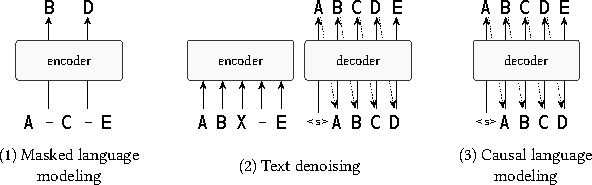
\includegraphics[width=0.9\textwidth]{img/objectives.pdf}
    \caption{A scheme of the common objectives used by pretrained models: (1) masked language modeling (encoder-only), (2) text denoising (encoder-decoder), (3)  causal language modeling (decoder-only). The special symbol \texttt{<s>} (beginning of a sentence) is used to bootstrap the decoding process.}\label{fig:objectives}
\end{figure*}


\paragraph{Finetuning} By \emph{finetuning} a model, we mean additional training of a pretrained model on a task-specific dataset. Finetuning is more efficient than training a model from scratch, but it is only a one-time process: repeated model updates can lead to erasing previous knowledge, also known as ``catastrophic forgetting'' \cite{mccloskey1989catastrophic,kirkpatrick2017overcoming}. This problem is partially mitigated by multi-task finetuning, in which the tasks are unified under a pre-specified input format and the model is finetuned for all the tasks at once \cite{sanh2021multitask,xieUnifiedSKGUnifyingMultiTasking2022}.


\paragraph{Few-shot and Zero-shot Settings} If the size of the finetuning data is very limited (under \textasciitilde 100 examples), we talk about \emph{few-shot} setting. By limiting the finetuning data to zero, we arrive at a \emph{zero-shot} setting, in which we use a model on the task which it has not been trained for. These settings are crucial for tasks with scarce data, also called \emph{low-resource scenarios} \cite{hedderich2021survey}.

\paragraph{Text Generation} For generating text from a transformer decoder, we can use \textit{left-to-right autoregressive decoding} \cite[p.196]{jurafsky2024}. The decoding process starts by feeding a special \texttt{<s>} (beginning of sequence) token into the decoder and then iteratively selecting the \emph{i}-th token based on the probability distribution for the \emph{i}-th position until the  \texttt{</s>} (end of sequence) token is decoded. The procedure is outlined in Algorithm \ref{alg:decoding}.
\begin{algorithm}[ht]
    \begin{algorithmic}[1]
        \State{Initialize: $Y= \texttt{<s>}, y = \texttt{<s>}$ \Comment{Output sequence, current token}}
        \While{$y \neq \texttt{</s>}$}
        \State Predict next token probability distribution: $p(y | Y)$
        \State Select the next token: $y \sim p(y | Y)$ \label{alg:dec:sample}
        \State Update output sequence: $Y = Y \cup y$
        \EndWhile
        \State Return $Y$
    \end{algorithmic}
    \caption{Autoregressive decoding}
    \label{alg:decoding}
\end{algorithm}

\noindent The sampling step (line \ref{alg:dec:sample}) can be realized in various ways, including:
\begin{itemize}
    \item \textbf{Greedy decoding}: Select the most probable token: $y_i = \argmax{y \in V} p_\theta(y|\mathbf{y}_{<i}).$
    \item \textbf{Top-$k$ sampling}: Sample the next token from the $k$ most probable tokens.
    \item \textbf{Top-$p$ (nucleus) sampling} \cite{holtzman2019curious}: Sample the next token from the tokens with cumulative probability $p$.
    \item \textbf{Beam search}: Extend the $k$ most probable sequences from the previous step with the next tokens, and select the $k$ most probable sequences for the next step.
\end{itemize}
While greedy decoding and beam search are used to generate more probable sequences (approximating the algorithm for estimating the most probable sequence, which has exponential complexity), sampling algorithms are used to decode more creative outputs.\footnote{The list of the decoding algorithms as presented here is not exhaustive; see \citet{zarriess2021decoding} and \citet{wiher2022decoding} for an overview and further discussion.}

\subsection{Large Language Models}
\label{sec:llms}
Scaling the models in terms of the number of parameters and the size of the training data has turned out to further improve the performance of the models \cite{kaplan2020scaling,hoffmann2022training}. Larger models were shown to exhibit unprecedented capabilities in terms of language fluency, language understanding, and reasoning skills \cite{wei2022emergent,bubeck2023sparks}, giving name to a specific category of \emph{\aclp{llm} (\acsp{llm}\glsunset{llm};} \citealp{brown2020language,zhao2023survey}). Broadly speaking, \acp{llm} are larger than 1B parameters and based on the transformer decoder architecture. In many \ac{nlp} tasks---from document-level translation \cite{wang2023documentlevel} and \ac{mt} evaluation \cite{kocmiLargeLanguageModels2023}, to news summarization \cite{zhang2024benchmarking} and story generation \cite{xie2023next}---\acp{llm} have comparable or better performance than previous task-specific approaches developed over last decades.

\paragraph{In-context Learning} \acp{llm} can perform novel tasks without the need for finetuning on task-specific data. Instead, the task can be defined by giving examples in the \emph{prompt}, i.e., the text used as a decoding prefix. By considering the input-output examples in the task of causal language modeling, the model can learn the task specification without any further training. This ability is known as \emph{in-context learning} \cite{brown2020language,dong2022survey}. If the model is given a limited set of input-output examples in the prompt, we talk about \emph{few-shot prompting}; if the model is given no examples, we talk about \emph{zero-shot prompting}.

\paragraph{Instruction Tuning} The key to strong cross-task performance of \acp{llm} is instruction tuning: finetuning on a large dataset of tasks formulated using natural language instructions, such as \textit{``Answer this question: \{question\}''} or \textit{``Translate this sentence: \{sentence\}''} \cite{sanh2021multitask,ouyang2022TrainingLM}. Due to their strong generalization abilities, the instruction-tuned models can be easily prompted to perform a task of choice in natural language, even without being directly trained for it.



\section{Data-to-Text Generation}
\label{sec:d2t}
In this section, we provide background for the task of \ac{d2t} generation. First, we present the \ac{d2t} applications (\autoref{sec:d2t-tasks}) and the subtasks to which \ac{d2t} generation can be decomposed (\autoref{sec:d2t-pipeline}). For the subtasks, we present rule-based (\autoref{sec:rule-d2t}), statistical (\autoref{sec:stat-d2t}), and neural (\autoref{sec:neural-d2t}) approaches. In the final part, we describe the datasets (\autoref{sec:datasets}) and evaluation metrics (\autoref{sec:evaluation}) we use in the thesis.

\subsection{Task and Applications}
\label{sec:d2t-tasks}

\ac{d2t} generation is an umbrella term for tasks that require transforming structured data into natural language. The input can take various forms, including graphs, trees, 2D tables, charts, or databases; the output is a fluent text that accurately conveys the information from the data \cite{gattSurveyStateArt2018,sharmaInnovationsNeuralDatatotext2022}.

Before we talk \ac{d2t} generation from the research point of view, let's have a look at its practical applications:

\begin{itemize}
    \item \textbf{Automated Journalism}: Augmenting (or, in simple cases, even replacing) human journalists for writing data-based reports, including:
          \begin{itemize}
              \item \textbf{News reports}: Automating news writing, e.g., for election results \cite{leppanen2017data}, incidents \cite{vanderleeCACAPODatasetMultilingual2020}, earthquakes \cite{oremus2014first}, or wildlife tracking \cite{siddharthan2012blogging,ponnamperuma2013tag2blog}.
              \item \textbf{Sport reports}: Generating game summaries for sports such as basketball \cite{wiseman2017challenges,thomson2020sportsett}, baseball \cite{puduppullyDatatotextGenerationEntity2019}, or soccer \cite{van2017pass}.
              \item \textbf{Financial reports}: Supporting financial decisions by generating comments on stock prices \cite{murakami2017learning,aoki2018generating} and summarizing financial documents \cite{chapman2022towards}.
              \item \textbf{Weather reports}: Generating weather forecasts and weather-related reports \cite{goldberg1994using,belz2005corpus,belz2008automatic,angeli-etal-2010-simple,balakrishnan2019constrained}.
          \end{itemize}
    \item \textbf{Business Intelligence Reports}: Providing decision support in business reports alongside data summaries and visualizations (mostly commercial companies such as \href{https://www.arria.com}{Arria}, \href{https://infosentience.com}{InfoSentience}, or \href{https://www.vphrase.com}{vPhrase}; see \citealp{daleNavigatingTextGeneration2023} for a recent overview).
    \item \textbf{Chart Captioning}: Generating captions\footnote{In contrast to image captioning \cite{stefanini2022show}, here the systems can rely on the underlying data in textual form (although the approaches can be hybrid, see e.g. \citealp{kantharajCharttoTextLargeScaleBenchmark2022}).} for charts or graphs, e.g., for assistive technologies, document indexing, or simplifying decision support \cite{demirGeneratingTextualSummaries2008,demirSummarizingInformationGraphics2012,obeidCharttoTextGeneratingNatural2020,kantharajCharttoTextLargeScaleBenchmark2022}.
    \item \textbf{Healthcare Summaries}: Providing clinical data summaries about patients to clinicians \cite{portet2009automatic,scott2013data}, or vice versa, providing medical information to patients, e.g., for behavioral change \cite{reiter2003lessons} or nutritional counseling \cite{balloccu-reiter-2022-comparing}.
    \item \textbf{Product Descriptions}: Automating generating product descriptions in specific domains such as for laptops and TVs \cite{wen2015toward,wen2016multi}, or general-domain approaches for big e-commerce platforms \cite{shaoControllableDiverseText2021,kotoCanPretrainedLanguage2022}.
\end{itemize}

\subsection{D2T Generation Pipeline}
\label{sec:d2t-pipeline}


Until recently, \ac{d2t} generation was decomposed into approximately 4-6 subtasks\footnote{The count is only approximate: for example, \citet{milleModD2TMultilayerDataset2023} further subdivides some of the subtasks, leading to 10 subtasks in total.} which were addressed separately \cite{reiterBuildingAppliedNatural1997,reiterArchitectureDatatoTextSystems2007,gattSurveyStateArt2018}. Even though the recent advances enable approaches which solve the task in \emph{end-to-end} fashion (i.e., without intermediate steps), the subtasks are still relevant for conceptualization of \ac{d2t} generation. We selected the following five representative subtasks illustrated in \autoref{fig:pipeline}:

\begin{enumerate}
    \item \textbf{Content Selection}: Deciding which facts from the structured data
          to include in the text.
    \item \textbf{Document Planning}: Determining the order of the
          facts, dividing the facts into paragraphs.
    \item \textbf{Sentence Planning}: Aggregating the facts into
          sentences.
    \item \textbf{Lexicalisation}: Transforming the facts to text segments.
    \item \textbf{Surface Realisation}: Combining the text segments into a well-formed text in natural language.
\end{enumerate}


\begin{figure*}[t]
    \centering
    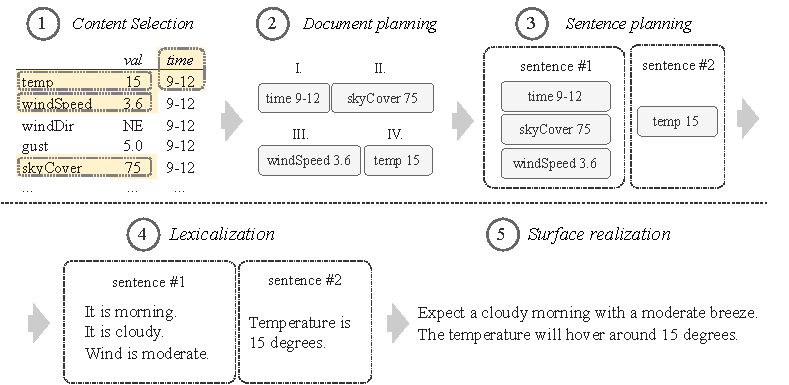
\includegraphics[width=\textwidth]{img/pipeline.pdf}

    \caption{A five-step \ac{d2t} generation pipeline on the example of generating a weather forecast. (1) The relevant fields for the forecast are selected from the data table. (2) The fields are ordered. (3) The ordered fields are aggregated into sentences. (4) Each field is transformed into a text segment. (5) The text segments are combined into the final text.}\label{fig:pipeline}

\end{figure*}


Decomposing \ac{d2t} generation into subtasks helps to modularize the system. Each module can have a specific and well-defined function, which makes the system more explainable. Modularization also enables realizing each subtask using a different approach (see \Cref{sec:rule-d2t,sec:stat-d2t,sec:neural-d2t}).

The subtasks are typically executed in a \emph{pipeline}, i.e., the input is sequentially processed by a series of modules. The main issue of the pipeline-based approach is error accumulation: the errors from one module propagating to downstream modules. Despite this issue, the pipeline approach remains widely used. It can also benefit end-to-end neural systems \cite{ferreiraNeuralDatatotextGeneration2019}, as we will explore in \autoref{sec:pipeline}.


\subsection{Rule-based Approaches}
\label{sec:rule-d2t}

By \emph{rule-based approaches} for \ac{d2t} generation, we mean the approaches using manually defined rules or grammars (as opposed to data-driven approaches in \Cref{sec:stat-d2t,sec:neural-d2t}, in which the system inner workings are derived from the data). Rule-based approaches, in combination with other approaches, are still in use in various forms today \cite{gattSurveyStateArt2018,daleNaturalLanguageGeneration2020,daleNavigatingTextGeneration2023}. It is helpful to view these approaches through the lens of the \ac{d2t} generation pipeline (\autoref{sec:d2t-pipeline}), as these approaches typically tackle particular subtasks of the pipeline.


\paragraph{Content Selection}
Extracting meaningful information from the data typically relies on domain-specific heuristics, e.g., \textit{``if a pattern is detected in the signal, include it in the report''} \cite{portet2009automatic}. Various factors can influence the decision, including the target length of the report, the type of the report, and its target audience \cite{gkatziaContentSelectionDatatoText2016}.

\paragraph{Text Planning} Rule-based text planning follows discourse strategies, which are designed to satisfy the desired communicative goals (such as \emph{define}, \emph{compare}, or \emph{describe}; \citealp{mckeown1985text}). The resulting rules are typically in the form \textit{``if a player scores two consecutive goals, describe these in the same sentence''}  \cite{gattSurveyStateArt2018}.


\paragraph{Template-based Lexicalization}
Simpler rule-based approaches for lexicalization and surface realization are typically based on \emph{templates}: pre-written text snippets which are filled with values from the data. Templates can range from simple fill-in-the-blank approaches (such as \textit{``The temperature will be \{temp\} degrees''}) to more sophisticated templates using a templating language \cite{gatt2009simplenlg,reiter2016nlg}.  Rules are used for selecting the templates, combining them, and filling the placeholders with values (the last being non-trivial in languages with rich morphology). The resulting rule-based system is usually tied to the specific task and domain, but it can be a way to generate sufficient outputs with reasonable development time and costs \cite{vanderleeAutomatedLearningTemplates2018}.


\paragraph{Grammar-based Lexicalization}
To handle more complex cases of lexicalization in rule-based systems, we can use grammar-based approaches. Even though a \emph{grammar} is technically also a set of rules, it differs by the fact that it describes the production rules for the whole sentence.
Grammar-based approaches are rooted in linguistic theories, such as systemic grammars \cite{halliday1985systemic,matthiessen1991lexico} or meaning-text theory \cite{mel1988dependency,goldberg1994using,milleModD2TMultilayerDataset2023}. The implementation typically relies on off-the-shelf realizers such as FUF/SURGE \cite{elhadad1997surge} or KPML \cite{bateman1997enabling}. Grammar-based approaches are more general-purpose than rule-based approaches; however, they require considerable manual effort, detailed input, and often also additional rules for choosing among related options \cite{gattSurveyStateArt2018}.
% FORGe \cite{milleFORGeWebNLG20172017,mille2019teaching}


\subsection{Statistical Approaches}
\label{sec:stat-d2t}
The idea of statistical\footnote{Since statistical \ac{d2t} generation approaches overlap with classical machine learning methods, these approaches are perhaps better described as \emph{pre-neural data-driven} approaches. However, we will stick to the more established term.} \ac{d2t} generation approaches is to \emph{estimate the parameters} of a system using a text corpus. This idea is not mutually exclusive with rule-based and grammar-based approaches; in fact, corpus statistics were initially used for re-ranking the outputs generated from a grammar-based system \cite{bangalore2000corpus,langkilde2000forest,ratnaparkhi2000trainable} or even integrated directly at the level of generation decisions \cite{belz2008automatic}.

Even entirely data-driven approaches still relied on grammatical rules; only the rules were derived from treebanks, i.e., text corpora annotated with syntactic and semantic sentence structures. For example, the approach of \citet{white2007towards} relied on a Combinatory Categorial Grammar \cite{steedman2001syntactic} derived from the Penn Treebank \cite{hockenmaier2007ccgbank}. There were also hybrid approaches which combined a set of hand-written rules or grammars with statistical models \cite{konstas2012concept,gardent2017statistical}.

The earlier stages of the \ac{d2t} generation pipeline, such as content selection or text planning, were usually tackled by \emph{unsupervised} machine learning methods. For example, \citet{duboue2003statistical} proposed to use a clustering-based method for content selection, estimating the relative importance of each cluster for the final text. \citet{barzilay2004catching} modelled the content structure using Hidden Markov Models \cite{baum1966statistical}, learning the structure from unannotated documents. For text planning, the approach of \citet{liang2009learning} used latent variables for learning alignment between the text and the data, which was used for text segmentation and structuring.

\subsection{Neural Approaches}
\label{sec:neural-d2t}
Building upon the previous data-driven approaches, neural networks (see \autoref{sec:nns}) started to be used more widely for \ac{d2t} generation around the year 2015 \cite{dusekTrainingNaturalLanguage2015,wen2015toward}. Thanks to advances in hardware \cite{hooker2021hardware} and capabilities of learning from large data \cite{lecun2015deep}, neural networks enabled not only building more powerful modules for the \ac{d2t} generation pipeline but also replacing the pipeline entirely with end-to-end models \cite{dusekEvaluatingStateoftheartEndtoEnd2020}. The field of neural \ac{d2t} generation has been gaining a lot of interest in recent years \cite{sharmaInnovationsNeuralDatatotext2022,lin2023survey}; here, we will mainly focus on the concepts and model architectures related to this thesis.


\paragraph{Linearization} For getting an input sequence suitable for the neural model, structured data first needs to be converted into a sequence of tokens. To preserve the data structure while keeping the input simple, a common practice is to \emph{linearize} the input: convert the data to a minimalistic representation with a handful of dedicated special tokens serving as delimiters. An example linearization of a knowledge graph is depicted in \autoref{fig:linearization}~(c). Linearization can be very effective \cite{yang2020improving,hoyle2021promoting,xieUnifiedSKGUnifyingMultiTasking2022}, beating specialized representations such as graph embeddings \cite{marcheggianiDeepGraphConvolutional2018,koncel-kedziorskiTextGenerationKnowledge2019}.

\begin{figure*}[h]
    \centering
    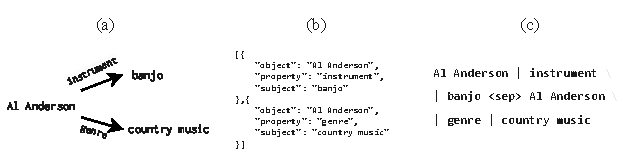
\includegraphics[width=\textwidth]{img/linearization.pdf}

    \caption{Representations of a simple knowledge graph: (a) the original knowledge graph, (b) JSON representation, (c) linearized representation.}\label{fig:linearization}

\end{figure*}

An alternative to linearization is to use special embeddings for the structural elements (e.g., for table rows and columns), which are summed with the positional and token embeddings \cite{wang2021tuta,yangTableFormerRobustTransformer2022}. Since the embeddings need to be learned, the approach is more suitable for high-resource tasks.

\paragraph{Delexicalization} A specific data value may appear only a few or zero times in the training data, making it difficult for the model to represent. Delexicalization is the process of replacing the values with placeholders, allowing the model to work only with the fill-in-the-blank templates \cite{oh2000stochastic,mairesse2010phrase,wen2015semantically,dusekSequencetoSequenceGenerationSpoken2016}. The values are filled in the post-processing step using simple rules. This approach was shown to be useful even for languages with rich morphology, where the values can be inflected using a dedicated language model \cite{duvsek2019neural}.

\paragraph{Sequence-to-Sequence Generation} Generating text from data in the end-to-end fashion, i.e., without intermediate steps, is enabled by neural \ac{seq2seq} models. \Ac{seq2seq} models are designed for transforming variable-length input sequences into variable-length output sequences \cite{cho2014learning,sutskever2014sequence}. The typical \ac{seq2seq} architecture is the encoder-decoder framework described in \autoref{sec:transformer}. In the case of \ac{d2t} generation, the input sequence is the linearized version of structured data, and the output sequence is the target text.

\paragraph{RNN-based Approaches} The original seq2seq approaches were designed for \ac{mt} \cite{cho2014learning,sutskever2014sequence}, but soon were also adopted for other \ac{nlg} tasks. \citet{wen2015semantically} use \acp{rnn} to generate the response in a dialogue system, using a structured representation of the dialogue act as the input. On a similar task, \citet{dusekSequencetoSequenceGenerationSpoken2016} show that instead of combining the model with a separate surface realization system, it is better to generate output strings directly with an \ac{rnn}. For generating weather reports, \citet{mei2016talk} use \acp{rnn} to address also the content selection step, identifying salient data records using the attention mechanism.

An important addition to the \ac{rnn}-based approaches was the \emph{copy mechanism}, which allows the model to generate the tokens by copying them from the input sequence \cite{gu2016incorporating,seeGetPointSummarization2017}. The copy mechanism is an alternative to delexicalization, delegating the job of filling the values to the model. Unlike delexicalization, the copy mechanism is trainable along with the rest of the model \cite{gehrmannEndtoEndContentPlan2018}.

\acp{rnn} were still used even after the introduction of the transformer model (\autoref{sec:transformer}), since they tend to work better in low-resource settings. For example, \citet{freitagUnsupervisedNaturalLanguage2018} experimented with using text denoising as an objective pretraining an \ac{rnn}-based system for \ac{d2t} generation. For adapting an \ac{rnn}-based model to other domains, \citet{wen2020recurrent} proposed \emph{data counterfeiting}, i.e., replacing delexicalized slots with slots from another domain. To improve the faithfulness of the outputs, \citet{rebuffel2021controlling} propose an architecture based on 3 \acp{rnn} computing content, faithfulness, and fluency scores. Various shared tasks and comparisons \cite{gardentWebNLGChallengeGenerating2017,dusekEvaluatingStateoftheartEndtoEnd2020,ferreiraNeuralDatatotextGeneration2019} showed that RNN-based approaches were generally competitive with rule-based approaches: the RNNs produce more fluent text, while the pipeline-based approaches made less semantic errors.


\paragraph{PLM-based Approaches} Using a transformer model for \ac{d2t} generation became practical with the arrival of \acp{plm}, which we have discussed in \autoref{sec:plms}. As an example, the 2020 WebNLG+ shared task (see \autoref{sec:datasets}) was dominated by systems based on pretrained encoder-decoder transformer models (\citealp{ferreira20202020,yang2020improving,agarwalMachineTranslationAided2020,kasnerTrainHardFinetune2020}).

\acp{plm} made it possible to get rid of both \emph{delexicalization} and \emph{copy mechanism}. The general knowledge of language, along with the learned ability to copy tokens from the input, allow the model to handle rare entities not present in the task-specific training data. \acp{plm} are also able to produce outputs with considerably better fluency than \ac{rnn}-based models. Moreover, the variants of \acp{plm} pretrained on multilingual corpora \cite{liuMultilingualDenoisingPretraining2020,xueMT5MassivelyMultilingual2021} are able to handle outputs in a variety of languages.

Due to the advantages above, \ac{plm}-based approaches excel in low-resource settings, which is a default setup for many \ac{d2t} generation tasks. Following \citet{chenFewShotNLGPreTrained2019}, other works adopted PLMs for few-shot or zero-shot D2T generation. In these scenarios, the models are typically finetuned on domain-specific data for few-shot generation \cite{changNeuralDatatoTextGeneration2021,suFewShotTabletoTextGeneration2021} or on the related domains for zero-shot generation \cite{kasner2022neural,kasnerMindLabelsDescribing2022}.

% The data representations are closely related to the particular datasets, which we discuss in \autoref{sec:datasets}. At the same time, the semantic accuracy is related to the evaluation metrics, which we discuss in \autoref{sec:evaluation}. 
Related work on \ac{plm}-based \ac{d2t} generation is discussed in detail in the recent surveys of \citet{sharmaInnovationsNeuralDatatotext2022} and \citet{lin2023survey}, to which we refer the reader for more information. Improving \ac{plm}-based \ac{d2t} generation in English revolves mainly around (1) finding suitable \emph{data representations} and (2) ensuring the \emph{semantic accuracy} of the outputs, which we will discuss in the following chapters.

\paragraph{LLM-based Approaches} At the time of writing, using \acp{llm} for \ac{d2t} generation is still in its naissance. The works that compared zero-shot or few-shot \ac{llm} prompting with finetuned \acp{plm} on existing datasets have found that the \acp{llm} rank behind state-of-the-art finetuned models on automatic metrics \cite{axelssonUsingLargeLanguage2023,yuanEvaluatingGenerativeModels2023}. In \autoref{sec:quintd}, we will also show that \acp{llm} can be employed for the zero-shot generation of data in standard data formats, the main issue still being the semantical accuracy of the outputs. However, there are yet no large-scale comparisons or attempts of finetuning \acp{llm} for \ac{d2t} generation.

% There are multiple factors which complicate benchmarking \acp{llm} on \ac{d2t} generation. Using closed \acp{llm}, which are accessible only through an API \cite{openai2023gpt4,chatgpt}, makes the work non-reproducible. Evaluation is also complicated with potential data contamination: the fact that any existing benchmark (including its test set) may have been included in the pretraining data of \acp{llm} \cite{golchin2023time,aiyappa-etal-2023-trust,balloccu2024leak}.

% On the other hand, \acp{llm} hold the promise of further simplifying data processing, enabling .

\subsection{Datasets}
\label{sec:datasets}

In this section, we outline the format and structure of \ac{d2t} generation datasets used in this thesis. The overview of the datasets is presented in \autoref{tab:datasets} (note that we mainly focus on the datasets in boldface).\footnote{We do not describe here our novel datasets presented in \citet{kasnerMindLabelsDescribing2022} and \citet{kasnerReferenceBasedMetricsAnalyzing2024}; these are described in their respective sections in \autoref{chap:investigating}.}

\begin{table*}[t]
    \centering\small
    \begin{tabular}{@{}lllr@{}}
        \toprule
        \textbf{Dataset}                                                                           & \textbf{Data Format} & \textbf{Domain(s)}      & \textbf{\# Ex.} \\  \midrule
        CACAPO \cite{vanderleeCACAPODatasetMultilingual2020}                                       & Key-value            & News$^\blacklozenge$    & 20,149          \\
        DART \cite{nan2021dart}                                                                    & \acs{rdf} triples    & Wikipedia$^\lozenge$    & 70,524          \\
        \textbf{E2E} \cite{dusekSemanticNoiseMatters2019,dusekEvaluatingStateoftheartEndtoEnd2020} & Key-value            & Restaurants             & 36,856          \\
        EventNarrative \cite{colas2021eventnarrative}                                              & \acs{rdf} triples    & Events$^\lozenge$       & 224,428         \\
        HiTab \cite{chengHiTabHierarchicalTable2021}                                               & Table w/hl           & Statistics$^\lozenge$   & 10,672          \\
        Chart-To-Text \cite{kantharajCharttoTextLargeScaleBenchmark2022}                           & Table                & Statistics$^\lozenge$   & 34,811          \\
        Logic2Text \cite{chenLogic2TextHighFidelityNatural2020}                                    & Table w/hl           & Wikipedia$^\lozenge$    & 10,753          \\
        LogicNLG \cite{chenLogicalNaturalLanguage2020}                                             & Table                & Wikipedia$^\lozenge$    & 37,015          \\
        NumericNLG \cite{suadaaTabletoTextGenerationNumerical2021}                                 & Table                & Science$^\lozenge$      & 1,355           \\
        SciGen \cite{moosaviLearningReasonText2021}                                                & Table                & Science$^\lozenge$      & 17,551          \\
        \textbf{Rotowire}$^*$ \cite{wiseman2017challenges}                                         & Table                & Basketball              & 6,150           \\
        ToTTo \cite{parikhToTToControlledTableToText2020}                                          & Table w/hl           & Wikipedia$^\lozenge$    & 136,553         \\
        \textbf{WebNLG} \cite{gardentWebNLGChallengeGenerating2017}                                & \acs{rdf} triples    & DBPedia$^\blacklozenge$ & 42,873          \\
        WikiBio \cite{lebretNeuralTextGeneration2016}                                              & Key-value            & Biographies$^\lozenge$  & 728,321         \\
        WikiSQL \cite{zhong2017seq2sql}                                                            & Table + SQL          & Wikipedia$^\lozenge$    & 80,654          \\
        WikiTableText \cite{bao2018table}                                                          & Key-value            & Wikipedia$^\lozenge$    & 13,318          \\
        \bottomrule
    \end{tabular}
    \caption{The list of \ac{d2t} datasets used in this work. All the datasets are included in the \textsc{TabGenie} framework (\autoref{sec:tabgenie}), except for Rotowire, where we include instead its updated version SportSett:Basketball \cite{thomson2020sportsett}. The datasets in \textbf{boldface} are also used in other experiments. Glossary of data types: \textit{Key-value}: key-value pairs, \textit{Graph}: subject-predicate-object triples, \textit{Table}: tabular data (\textit{w/hl}: with highlighted cells), \textit{Chart}: chart data, \textit{SQL}: strings with SQL queries. $\blacklozenge$ indicates that the dataset is multi-domain; $\lozenge$ indicates that the dataset is open-domain.}
    \label{tab:datasets}.
\end{table*}

\paragraph{Data Formats} The following formats of structured data are present in our datasets:

\begin{itemize}
    \item \textbf{Key-value pairs}: The input is a set of tuples $(k, v)$, where $k$ is a key (also called a slot), which is typically a text string, and $v$ is a value, which can be a text string or a number. The format is often used as a \emph{\ac{mr}} in dialogue systems, e.g., for representing dialogue states or dialogue acts \cite{rastogiScalableMultiDomainConversational2020,budzianowskiMultiWOZLargeScaleMultiDomain2020}.
    \item \textbf{\acs{rdf} (\Acl{rdf}\glsunset{rdf})\footnote{See \url{https://www.w3.org/TR/PR-rdf-syntax/}.} triples}: The input is a set of triples $(s, p, o)$, where $s$ is a \emph{subject},  $p$ is a \emph{predicate}, and $o$ is an \textit{object}. This formalism directly translates to a \emph{directed graph}, where $s$ and $o$ are nodes, and $p$ is a directed edge between these nodes. In a knowledge graph such as Wikidata or DBPedia, the subject is usually an entity (e.g., a person, an object, or a place); the object is either also an entity or a generic value. The predicate expresses the relation between the subject and the object.
    \item \textbf{Table}: The input is structured as a \textit{table}, i.e., a two-dimensional cell matrix of $m$ columns and $n$ rows. A table cell can contain a textual or numerical value. If a cell is marked as a heading, it contains the ``key'' for the respective row or column. In some datasets, a subset of cells is \emph{pre-highlighted} -- in that case, the output text should describe only that particular subset of cells. A generalized table may also contain merged cells, nested headings, or multiple disjoint table regions (analogically to real-world data).
\end{itemize}

As we show in \autoref{chap:tabgenie}, key-value pairs and RDF triples can be converted to a tabular format with minimal information loss. In \autoref{sec:quintd}, we also show how to handle data in the JSON\footnote{JavaScript Object Notation; see \url{https://www.json.org}.} format, which is standardly not used as an input format in \ac{d2t} generation datasets. We do not consider here data formats with a more task-specific structure such as \acl{amr} (\acs{amr}\glsunset{amr}; \citealp{banarescu2013abstract}).

\paragraph{Domains} In \ac{d2t} generation, the notion of a \emph{domain} is mostly used in the sense ``an area of interest''.\footnote{\url{https://dictionary.cambridge.org/dictionary/english/domain}} However, its exact scope may vary: while \citet{wen2016multi} consider the domains of TVs and laptops as distinct, \citet{lin2023survey} propose a single domain ``tables from ACL Anthology papers'' \cite{suadaaTabletoTextGenerationNumerical2021}. The definition becomes more apparent in relation to the term \emph{multi-domain}: most commonly, a dataset is called \emph{multi-domain} if two subsets of data come from distributions so different that the model trained on one subset does not straightforwardly generalize to the second \cite{vanderleeCACAPODatasetMultilingual2020,budzianowskiMultiWOZLargeScaleMultiDomain2020,rastogiScalableMultiDomainConversational2020}. If the topic of the dataset is unrestricted, or if it is based on a large-scale data source such as Wikipedia, the dataset is considered \emph{open-domain} (see, e.g., \citealp{chenLogicalNaturalLanguage2020,nan2021dart,kann2022open}).

\paragraph{Datasets} The following \ac{d2t} generation datasets are the most relevant for the thesis:

\begin{itemize}
    \item \textbf{WebNLG}: The WebNLG dataset \cite{gardentCreatingTrainingCorpora2017,gardentWebNLGChallengeGenerating2017} contains \ac{rdf} triples from DBPedia \cite{auer2007dbpedia} and their crowdsourced descriptions. Each example consists of 1-7 triples, forming a subgraph in the DBPedia knowledge graph. The target text should describe all the entities and the relations between them. The original WebNLG dataset \cite{gardentCreatingTrainingCorpora2017} contains 15 domains, out of which 5 are \emph{unseen}, i.e., included only in the test set. Each set of triples included several verbalizations to promote lexical variability. In version 2, the dataset has been fixed, annotated for intermediate subtasks, and enriched with semi-automated German translations \cite{shimorinaHandlingRareItems2018,castroferreiraEnrichingWebNLGCorpus2018}. Version 3 \cite{ferreira20202020} contains one additional domain and automatic translations to Russian.
          \begin{itemize}
              \item
                    We participated in the 2020 edition of \emph{WebNLG Challenge}, which is a series of shared tasks based on the WebNLG dataset (\citealp{gardentWebNLGChallengeGenerating2017,shimorinaWebNLGChallengeHuman2019,ferreira20202020,cripwell2023WebNLGShared2023}; see \autoref{sec:finetuning}). We also used the dataset in the experiments on low-resource \ac{d2t} generation (\Cref{sec:iterative,sec:pipeline}), evaluation (\autoref{sec:sem-acc}), data processing (\autoref{sec:tabgenie}), and out-of-domain generalization (\autoref{sec:rel2text}).
          \end{itemize}

    \item \textbf{E2E}: The E2E dataset \cite{dusekEvaluatingStateoftheartEndtoEnd2020,dusekSemanticNoiseMatters2019} contains restaurant descriptions in the form of key-value pairs (3-8 items per example) and corresponding human-written restaurant recommendations. The name of the dataset is derived from the E2E Challenge, a shared task that focused on evaluating end-to-end \ac{d2t} generation systems \cite{dusekEvaluatingStateoftheartEndtoEnd2020}. Since the original version of the dataset contained semantic noise (incorrect or missing facts in the crowdsourced descriptions), we use the cleaned version from \citet{dusekSemanticNoiseMatters2019} as the default version for our experiments.
          \begin{itemize}
              \item
                    Similarly to WebNLG, we used the dataset in the experiments on low-resource \ac{d2t} generation (\Cref{sec:iterative,sec:pipeline}), evaluation (\autoref{sec:sem-acc}), and data processing (\autoref{sec:tabgenie}).
          \end{itemize}

    \item \textbf{Rotowire}: Rotowire \cite{wiseman2017challenges} is a dataset with tabular statistics of basketball games and their corresponding game summaries. The target text contains only a small subset of the full input table, which is not highlighted a priori, so the systems also need to model the content selection step. Together with the above-average length of the target summaries, this aspect makes the dataset particularly challenging for \ac{d2t} generation systems.
          \begin{itemize}
              \item
                    We used the outputs from the neural systems on this dataset for building a token-level evaluation metric (\autoref{sec:tok-eval}). We also included its updated version SportSett:Basketball \cite{thomson2020sportsett} in our data processing toolkit (\autoref{sec:tabgenie}).
          \end{itemize}
\end{itemize}



\subsection{Evaluation Metrics}
\label{sec:evaluation}

The most common evaluation measures for \ac{d2t} generation are \emph{intrinsic}, i.e., focusing on evaluating certain aspects of the quality of the system and its outputs \cite{gkatzia2015snapshot,celikyilmazEvaluationTextGeneration2021}.\footnote{As opposed to \emph{extrinsic} measures, which evaluate the impact of the system in the external environment \cite{celikyilmazEvaluationTextGeneration2021}. While \emph{extrinsic} metrics could give us a better picture of the real-world impact, they are not suitable for early research stages due to high demands on the system quality, and they are also less suitable for evaluating individual subtasks \cite{van2019best}.} The intrinsic measures can be grouped between \emph{automatic metrics} and \emph{human evaluation}. Automatic metrics are generally cheaper, faster, and more replicable. However, they mostly serve only as a crude heuristic for the desired performance measure. Human evaluation is more expensive and difficult to execute, but if executed correctly, it can give us a more precise and fine-grained picture of system performance. A rule of thumb is that an experimental result should be supported by both kinds of metrics.


If we have human-written (also called \emph{ground truth} or \emph{golden}\footnote{The term \emph{golden} can misleadingly suggest that human-written references are the ``holy grail'' which the systems should imitate. This is generally an overstatement, human-written references are often noisy and faulty \cite{dusekSemanticNoiseMatters2019,clarkAllThatHuman2021}.}) reference texts at our disposal, we can use \emph{reference-based}  automatic metrics. The implicit assumption with reference-based metrics is that the more similar the generated text is to the respective human-written reference text, the better. \emph{Referenceless} metrics, on the other hand, can be more varied: they can either judge the intrinsic qualities of the text, such as text fluency, text diversity, and reading level, or---taking the input data into account---the faithfulness of the text with respect to the input data.


\paragraph{Lexical Similarity} Lexical similarity metrics measure the similarity between the generated and reference text using word-level overlap. The metrics are fast, easy to compute, and have been used for decades as a convenient proxy for system comparison in various \ac{nlp} areas \cite{celikyilmazEvaluationTextGeneration2021}. However, there is a recent upsurge of works arguing against these metrics because their correlations with human judgments for high-quality outputs are low or negative, and the metrics fail to capture fine-grained phenomena \cite{mathurTangledBLEUReevaluating2020,kocmiShipNotShip2021,gehrmannRepairingCrackedFoundation2022}. As a general rule, lexical similarity metrics (if used, e.g., for comparison with prior work) should be accompanied by other metrics.

Here are some of the common metrics which we use in this work:

\begin{itemize}
    \item \textbf{BLEU} \cite{papineni2002bleu} measures $n$-gram precision, i.e., to which extent do the $n$-grams in the generated text correspond to the reference text.  It is computed as a geometric mean of the $n$-gram precisions, with a brevity penalty to penalize shorter outputs. BLEU was originally used for evaluating \ac{mt}, but it has become commonplace in \ac{nlp}. The SacreBLEU library \cite{post2018call}  was developed to tackle inconsistencies in implementations of the metric.
    \item \textbf{ROUGE} \cite{lin-2004-rouge} is a set of metrics that focus on recall, i.e., to which extent does the generated text preserve the information in the reference text. ROUGE has been originally designed for evaluating automatic summarization, but similarly to BLEU, it has been used widely (and as recently found by \citet{gruskyRogueScores2023}, oftentimes incorrectly) across the \ac{nlp} literature. ROUGE includes several variants, such as ROUGE-L, which measures the longest matching word sequence, and ROUGE-{1/2/3/4}, which measures the overlap on the respective $n$-grams.
    \item \textbf{METEOR} \cite{banerjee-lavie-2005-meteor} is a metric that computes the harmonic mean of precision and recall computed on unigrams. METEOR also partially addresses semantic similarities of texts by using stemming and synonym matching. It has been shown to produce better correlations with human judgments than BLEU \cite{agarwal2008meteor} but is more complex and expensive to compute.
    \item \textbf{NIST} \cite{martin2000nist} is a metric which focuses on precision similarly to BLEU. However, it assigns lower weights to less common n-grams, which are considered less informative \cite{doddington2002automatic}. Its length penalty is also more robust to slight variations in text length.
    \item \textbf{ChrF++} \cite{popovic2015chrf,popovic2017chrf} is a metric which computes the F1-score on \emph{character} $n$-grams. The metric is more robust to morphological variations than word-level metrics. On top of the original ChrF metric, Chrf++ also considers word unigrams and bigrams along with the character $n$-grams.
          % \item \textbf{CIDEr} \cite{vedantam2015cider} is a metric originally designed for evaluating image captions. It considers n-gram overlap, word frequency, and the informativeness of the generated caption compared to the reference captions. While not typically used for text summarization or \ac{mt} evaluation, it can be adapted for these tasks as well.
\end{itemize}
\paragraph{Semantic Similarity} As described in \autoref{sec:text-repr}, word embeddings map words with similar meanings to the shared part of the vector space. Semantic similarity metrics use this fact to measure the similarity of the texts as a distance between their embeddings. The metrics most often rely on \emph{contextual embeddings} computed by pretrained \ac{rnn} or transformer encoders (\citealp{peters2018deep,devlinBERTPretrainingDeep2019}; see \autoref{sec:transformer}). In contrast with lexical similarity metrics, semantic similarity metrics are more robust to the lexical variations but are more computationally expensive. They are also subject to the limitations of pretrained models, including their biases and black-box nature.

The following are the metrics which we use in this work:

\begin{itemize}
    \item \textbf{BERTScore} \cite{zhang2019bertscore} measures the semantic similarity of the texts by computing cosine similarity between the embeddings of the texts encoded by a pretrained transformer model. It was initially developed on top of BERT \cite{devlinBERTPretrainingDeep2019}, but it now supports other transformer encoder models. Its flexibility helps to achieve better correlations with human judgment but makes it less suitable for intra-work comparison.
    \item \textbf{BLEURT} \cite{sellam2020bleurt} measures semantic similarity using a BERT model \cite{devlinBERTPretrainingDeep2019} which is further finetuned on synthetically labeled data. The similarity is computed as a cosine similarity of the contextual embeddings. Compared to BERTScore, BLEURT is less flexible but ensures a more consistent setup across works.
    \item \textbf{NUBIA} \cite{kaneNUBIANeUralBased2020} measures semantic equivalence of texts by combining features from two finetuned RoBERTa models \cite{liuRoBERTaRobustlyOptimized2019}, on the semantic similarity benchmark STS \cite{cer-etal-2017-semeval} and on the natural language inference benchmark MNLI \cite{williams2018mnli}; along with the perplexity from the GPT-2 model \cite{radford2019language}. These features are combined using an \ac{mlp} layer. Combining the features ensures better robustness of the metric at the cost of higher complexity and higher computational requirements.
\end{itemize}

\paragraph{Semantic Accuracy} Semantic accuracy---also called \emph{faithfulness} or \emph{factual consistency} \cite{celikyilmazEvaluationTextGeneration2021}---measures inaccuracies in the output text with respect to the input data. The inaccuracies can be broadly divided into \emph{omissions} (the model not mentioning facts in the input data) and \emph{hallucinations} (the model mentioning extra facts that are not supported by the input data). Naturally, omissions apply only if the task requires mentioning all the facts in the input data. Further, the hallucinations can be \emph{extrinsic}, i.e., the model introduces external information not present in the data, or \emph{intrinsic}, i.e., the model uses the data incorrectly \cite{maynezFaithfulnessFactualityAbstractive2020}.

There are no widely accepted metrics for measuring semantic accuracy in \ac{d2t} generation. The closest notion is the \emph{slot error rate} from task-oriented dialogue systems, which is typically implemented by exact string match or regular expressions  \cite{wen2015semantically,dusekEvaluatingStateoftheartEndtoEnd2020}. For tabular data, PARENT \cite{dhingraHandlingDivergentReference2019} was proposed as a reference-based metric, which uses lexical alignment models for computing precision and recall for tabular values.  In \Cref{sec:sem-acc,sec:tok-eval}, we present two novel \emph{referenceless} metrics for evaluating semantic accuracy of \ac{d2t} generation using \acp{plm}. In \autoref{sec:quintd}, we also show how to evaluate the semantic accuracy of texts using a prompted \ac{llm}.

\paragraph{Text Fluency} Text fluency is a catch-all term for measuring grammatical correctness, spelling, word, and stylistical choices of text \cite{celikyilmazEvaluationTextGeneration2021}. Since texts that are more similar to human written text tend to be more fluent, lexical and semantic similarity metrics (such as BLEU) are often used as a proxy for measuring text fluency. Alternatively, we can use the \emph{perplexity} of the text under a neural \ac{lm}. This approach assumes that the \ac{lm} assigns lower probability to less probable sentences \cite{leeFactualityEnhancedLanguage2022,kaneNUBIANeUralBased2020}.


\paragraph{Lexical Diversity} Lexical diversity measures the variability and richness of expressions in the text \cite{vanmiltenburgMeasuringDiversityAutomatic2018}. One way to express lexical diversity is the ratio between the average number of different words and the total number of words, called \emph{\ac{ttr}} or \emph{distinct $n$-grams} \cite{johnson1944studies,li2016diversity}. Another way is to measure conditional entropy of $n$-grams \cite{shannon1948mathematical}.
Lexical diversity is not generally required for \ac{d2t} generation, although there are approaches explicitly aiming to decode diverse outputs \cite{hanGeneratingDiverseDescriptions2021,perlitzDiversityEnhancedTabletoText2022}.

\paragraph{Human Evaluation} Since automatic metrics serve only as imperfect proxies for human judgment, using human annotators is a crucial part of any \ac{nlg} experimental evaluation \cite{gehrmannRepairingCrackedFoundation2022}. Although there are attempts at standardizing human evaluation \cite{thomsonGoldStandardMethodology2020}, human annotation protocols are usually task-specific \cite{van2019best,belzDisentanglingPropertiesHuman2020}. There are two main paradigms of human evaluation: large-scale evaluation using crowd workers mainly focusing on quantitative aspects (\emph{crowdsourcing}), and small-scale evaluation using expert annotators focusing primarily on qualitative aspects (\emph{manual evaluation}).

\begin{itemize}
    \item \textbf{Crowdsourcing}: Crowdsourcing platforms such as Amazon Mechanical Turk\footnote{\url{https://www.mturk.com}} or Prolific\footnote{\url{https://prolific.com}} are often used for distributing the work between human annotators. These platforms offer a convenient interface for hiring annotators with a specific background. Due to financial incentives, the quality of outputs may vary, especially if the workers are tempted to delegate the task at hand to \acp{llm} \cite{veselovskyArtificialArtificialArtificial2023}. It is, therefore, necessary to employ quality assurance checks in the annotation process.
    \item \textbf{Manual Evaluation}: To measure fine-grained aspects of output quality, manual evaluation can be performed by the paper authors or other domain experts on a small or moderate-sized sample of data (20-100 examples). The main goal of manual evaluation is to provide insights into the kinds of errors that appear in the output texts.
\end{itemize}


\paragraph{LLM-based Evaluation} Recently, researchers have started to examine the potential of replacing human workers with \acp{llm} \cite{zhaoInvestigatingTabletoTextGeneration2023,sottanaEvaluationMetricsEra2023,kocmiLargeLanguageModels2023,chiang-lee-2023-large,wangChatGPTGoodNLG2023a,fu2023gptscore}. In particular, the GPT-4 model \cite{openai2023gpt4} was shown to be capable of following fine-grained instructions compared to other LLMs and of having high correlations with human judgment on evaluating generated texts.  Since the model can be prompted for the specific task, using \acp{llm} can be cheaper and more robust than human annotators. However, due to concerns about its non-reproducibility \cite{kocmiGEMBAMQMDetectingTranslation2023} and bias \cite{wangLargeLanguageModels2023}, this evaluation method is only experimental.

